\documentclass[a4paper,12pt]{exam}
	\usepackage{graphicx}
	\usepackage[utf8]{inputenc}
	\usepackage[T1]{fontenc}
	\usepackage{listings}
	\usepackage{color}
	\usepackage{amsmath}
	\usepackage{enumerate}
	\usepackage{caption}
	\usepackage{subcaption}
	\definecolor{dkgreen}{rgb}{0,0.6,0}
	\definecolor{gray}{rgb}{0.5,0.5,0.5}
	\definecolor{mauve}{rgb}{0.58,0,0.82}

	\lstset{frame=tb,
	  language=Python,
	  aboveskip=3mm,
	  belowskip=3mm,
	  showstringspaces=false,
	  columns=flexible,
	  basicstyle={\small\ttfamily},
	  numbers=none,
	  numberstyle=\tiny\color{gray},
	  keywordstyle=\color{blue},
	  commentstyle=\color{dkgreen},
	  stringstyle=\color{mauve},
	  breaklines=true,
	  breakatwhitespace=true
	  tabsize=3
	}


\begin{document}
\begingroup 
	  \bf \Large Mecânica Clássica I\\
	  \indent \normalsize André Del Bianco Giuffrida
	\endgroup
	\\ \quad
	\\
	Exercício 28 Cap 4 - Symon
	\\ 
	\\
	As figuras de Lissajous são obtidas apartir das equações:\\
	\[
	 \begin{array}{ll}
	 x = A_x \cos{(\omega_x t + \theta_x)}, \quad \omega_x^2 =\frac{ k_x}{m}\\
	 y = A_y \cos{(\omega_y t + \theta_y)}, \quad \omega_y^2 =\frac{ k_y}{m}\\
	\end{array}
	\]
		\begin{figure}[wlh]
			\centering
			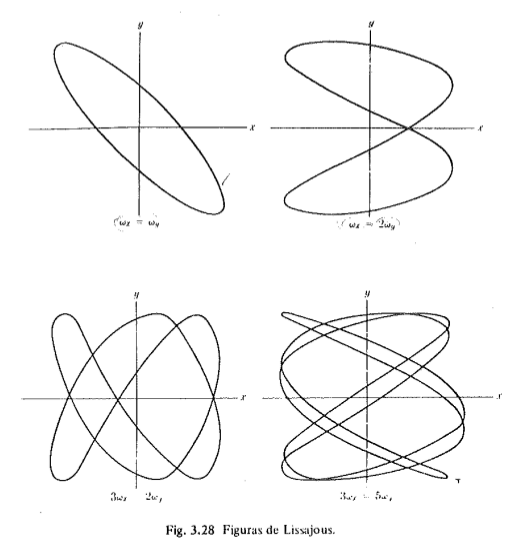
\includegraphics[scale=0.4]{Lissajous.png}
		\end{figure}
	\\
	Se $\theta_x = 0$ avalie $\theta_y$ para o caso em que $\omega_x = 2\omega_y$ :
	\[
	 \begin{array}{ll}
	 x = A_x \cos{(2\omega_y t )}\\
	 y = A_y \cos{(\omega_y t + \theta_y)}\\
	\end{array}
	\]
	Usando o código a seguir para plotar-mos as figuras:
	\begin{lstlisting}
		from math import *
		import sys
		import random
		pi = 3.141592
		#tempo para 1 periodo
		tmax = 2*pi
		#Resolucao
		resol = 0.001
		#Condicoes iniciais
		theta_y = 2*pi*random.random() #escolha aleatoria de theta_y
		theta_x = 0
		print str(theta_y)
		#Constantes
		Ax = 1
		Ay = 1
		Wx = 2
		Wy = 1
		for i in range(0,int(tmax/resol)):
			t = i*resol
			x = Ax*cos(Wx*t + theta_x)
			y = Ay*cos(Wy*t + theta_y)
			print x,y,t
	\end{lstlisting}
Obtemos:
			\begin{figure}[wlh]
			\centering
			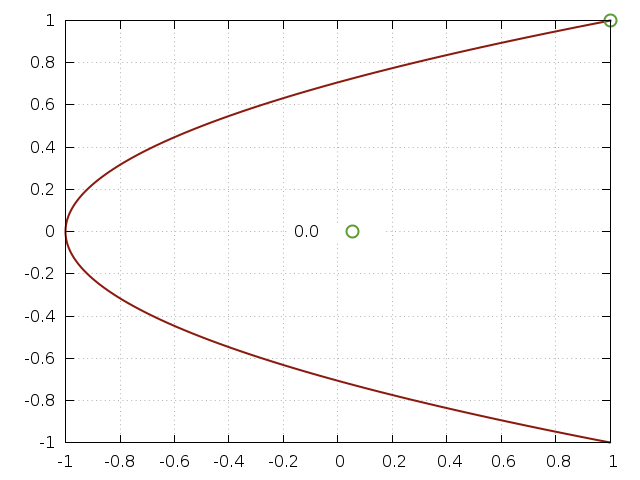
\includegraphics[scale=0.4]{4o0.png}
		\end{figure}
		
\end{document}		
